% We switch to portrait mode. This works as advertised.
\documentclass[a0,portrait]{a0poster}
% You might find the 'draft' option to a0 poster useful if you have
% lots of graphics, because they can take some time to process and
% display. (\documentclass[a0,draft]{a0poster})

%\usepackage[utf8]{inputenc}

% Switch off page numbers on a poster, obviously, and section numbers too.
\pagestyle{empty}
\setcounter{secnumdepth}{0}

%fonts
\usepackage[T1]{fontenc}
\usepackage{fontspec}
%\usepackage[oldstylenums, largesmallcaps]{kpfonts}
\setmainfont[Numbers=OldStyle]{Tex Gyre Pagella}
\setsansfont[BoldFont=Lovelo-LineBold]{Lovelo-LineBold}
%\renewcommand*\sfdefault{ugq}

\usepackage{hyperref}
\hypersetup{%
	pdftitle={Effects of a real world size distribution on the heterogeneous crystallisation of hard sphere colloids},%the title
	pdfauthor={Mathieu Leocmach},%your name
}

%proper math and math symbols
%\usepackage{amsmath}
\usepackage{amssymb}

\usepackage{siunitx}

\usepackage{multirow}

% Allow the usage of graphics (.jpg, .png, etc.) in the document
\usepackage{graphicx}
\usepackage{tikz}
\usetikzlibrary{arrows,shapes,backgrounds, positioning, intersections, decorations.markings, decorations.shapes, mindmap, shapes.geometric, matrix, patterns}

\usepackage{pgfplots}
%\usepgfplotslibrary{units}
\usepgfplotslibrary{groupplots}
\pgfplotsset{every axis/.append style={xlabel near ticks,ylabel near ticks}}
\pgfplotsset{every axis plot post/.append style={very thick}}

\usepgfplotslibrary{external}
%\tikzexternalize
%\tikzsetexternalprefix{fig_Rome/}
\tikzset{external/system call={lualatex \tikzexternalcheckshellescape -halt-on-error -interaction=batchmode -jobname "\image" "\texsource"}}

\usepackage{ragged2e}
\RaggedRight

\definecolor{Main}{rgb}{1, 0.66, 0}
\definecolor{Accent1}{rgb}{1,0.45,0}
\definecolor{Accent2}{rgb}{0.88,0.66,0}

% see documentation for a0poster class for the size options here
\let\Textsize\normalsize
\def\Head#1{\noindent\hbox to \hsize{\hfil{\LARGE\color{Main}\raggedright\textsf{#1}}}\bigskip}
\def\LHead#1{\noindent{\LARGE #1}\smallskip}
\def\Subhead#1{\noindent{\large\color{Accent1}\textsc{#1}}}
\def\Title#1{\noindent{\VeryHuge\color{Accent2}\raggedright\textsf{#1}}}

% The textpos package is necessary to position textblocks at arbitary 
% places on the page.
\usepackage[absolute,overlay,showboxes
]{textpos}
% Set up the grid
%
% Note that [40mm,40mm] is the margin round the edge of the page --
% it is _not_ the grid size. That is always defined as 
% PAGE_WIDTH/HGRID and PAGE_HEIGHT/VGRID. In this case we use
% 15 x 25. This gives us a wide central column for text (7 grid
% spacings) and two narrow columns (3 each) at each side for 
% pictures, separated by 1 grid spacing.
%
% Note however that texblocks can be positioned fractionally as well,
% so really any convenient grid size can be used.
%
\TPGrid[40mm,40mm]{15}{25}  % 3 - 1 - 7 - 1 - 3 Columns

% Mess with these as you like
\parindent=0pt
%\parindent=1cm
\parskip=0.5\baselineskip

\usepackage{paralist}

%bibliography
\usepackage{natbib}
\usepackage{bibentry}
\def\newblock{\hskip .11em plus .33em minus .07em}


%\includeonly{}

\begin{document}
%\tikzset{every mark/.append style={scale=0.8}}
%\pgfplotsset{every axis/.append style={small}}

\bibliographystyle{notitle}
%\nobibliography{sift}

% Understanding textblocks is the key to being able to do a poster in
% LaTeX. In
%
%    \begin{textblock}{wid}(x,y)
%    ...
%    \end{textblock}
%
% the first argument gives the block width in units of the grid
% cells specified above in \TPGrid; the second gives the (x,y)
% position on the grid, with the y axis pointing down.

% You will have to do a lot of previewing to get everything in the 
% right place.

% This gives good title positioning for a portrait poster.
% Watch out for hyphenation in titles - LaTeX will do it
% but it looks awful.
\begin{textblock}{15}(0,0)
\centering
\Title{
Wrinkling and yielding of protein gel
}

\LHead{Mathieu Leocmach}\qquad\texttt{\color{Accent1}mathieu.leocmach@polytechnique.org}\\
\LHead{Mathieu Nespoulous, Christophe Perge, Nicolas Taberlet, Thomas Gibaud,
Thibaut Divoux, Sébastien Manneville}

\LHead{\textsc{Laboratoire de Physique -- UMR 5672, Ecole Normale Supérieure de Lyon}}

\end{textblock}

\begin{textblock}{3}(0,2.5)
	\Head{Casein gel}
	
	In millipore water
	\begin{itemize}
	\item[4\%] Sodium caseinate (milk protein)\\
	Isoelectric point $\approx 4.6$
	\item[4\%] $\delta$-gluconolactone (\textsc{gdl})\\
	Slow hydrolysis into gluconic acid
	\end{itemize}
	
	\begin{tikzpicture}
	\begin{axis}[%
		xmin=0,
		ymin=0, ymax=7,
		xlabel={time (h)}, ylabel={\textcolor{Accent1}{pH}},
		extra tick style={grid=major},%
		extra y ticks={4.6}, extra y tick labels={},%
		axis y line*=left,
		width=0.7\textwidth,
		]
	\addplot+[no marks,Accent1] table[x expr={\thisrowno{0}/3600.+0.05}]{Y189_28800s.pH};
	\end{axis}
	\begin{axis}[%
		xmin=0,
		ymin=0,
		ylabel=\textcolor{Accent2}{$G^\prime$},
		axis y line*=right,
		axis x line=none,
		width=0.7\textwidth,
		]
	\addplot+[no marks,Accent2] table[x expr={\thisrowno{0}/3600.+0.05}]{Y235_28800s.prise};
	\end{axis}
	\end{tikzpicture}
\end{textblock}

\begin{textblock}{7}(4,2.5)
	\Head{Sealed cell}
	
	\tikzsetnextfilename{cell_brushes}
	\tikzset{external/force remake}
	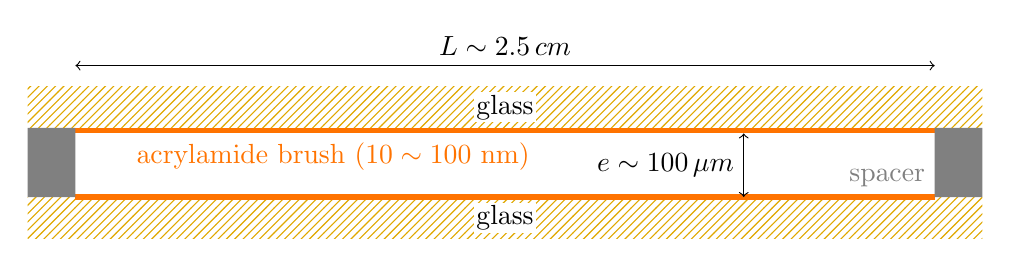
\begin{tikzpicture}
		\fill[pattern=north east lines,pattern color=Accent2] (0,0) rectangle (\textwidth,1.5em) node[midway,fill=white,inner sep=1pt] {glass};
		\fill[pattern=north east lines,pattern color=Accent2] (0,-2.5em) rectangle (\textwidth,-4em) node[midway,fill=white,inner sep=1pt] {glass};
		\draw[line width=2pt,Accent1] (0.05\textwidth,-2.5em) -- (0.95\textwidth,-2.5em) (0.05\textwidth,-1pt) -- (0.95\textwidth,-1pt) node[below,pos=0.30] {acrylamide brush ($10\sim 100$ nm)};
		\fill[gray] (0,0) rectangle (0.05\textwidth,-2.5em) (\textwidth,0) rectangle (0.95\textwidth,-2.5em) node[pos=1, above left] {spacer};
		\draw[<->] (0.75\textwidth,-2pt) -- (0.75\textwidth,-2.5em) node[midway,left] {$e\sim 100\,\mu m$};
		\draw[<->] (0.05\textwidth,2.25em) -- (0.95\textwidth,2.25em) node[midway,above] {$L\sim 2.5\,cm$};
	\end{tikzpicture}
	
	\begin{itemize}
	\item No adhesion on top and bottom (polymer brushes).
	\item Adhesion at the edge (solid spacers, no free interface)
	\end{itemize}
	
	\begin{tikzpicture}[inner sep=0, anchor=north west, thick]
	\node (a) {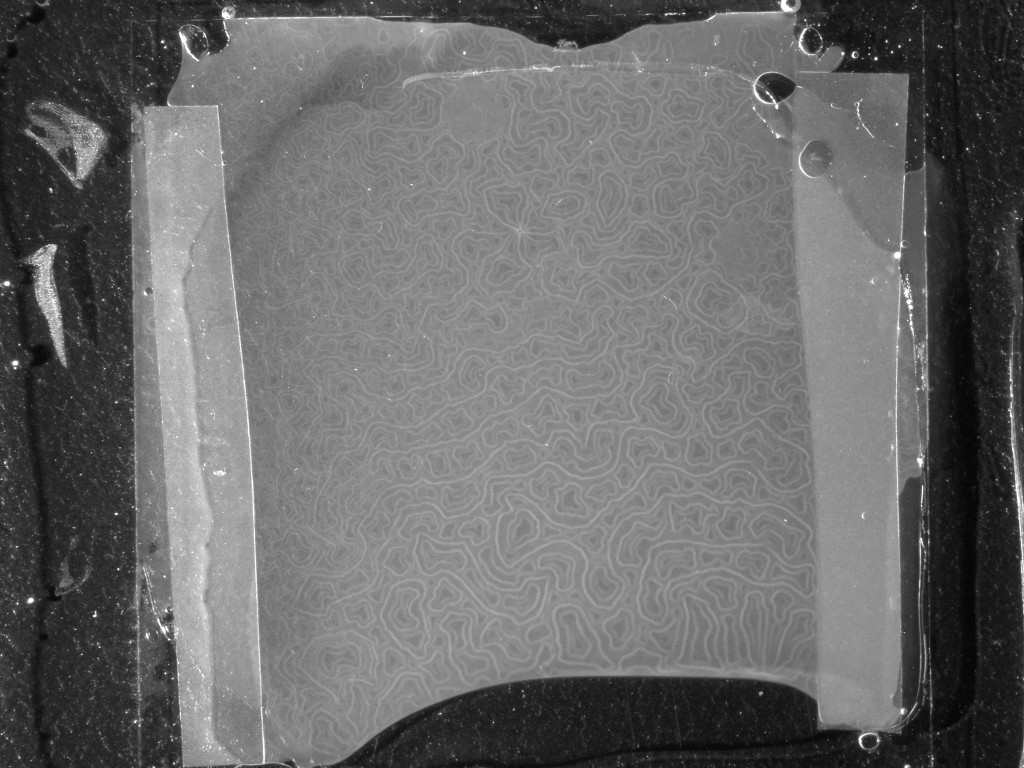
\includegraphics{cas3p2_fluo0p8_GDL4_50um_coating_2_zoom2}};
	\node at (a.north east) (b) {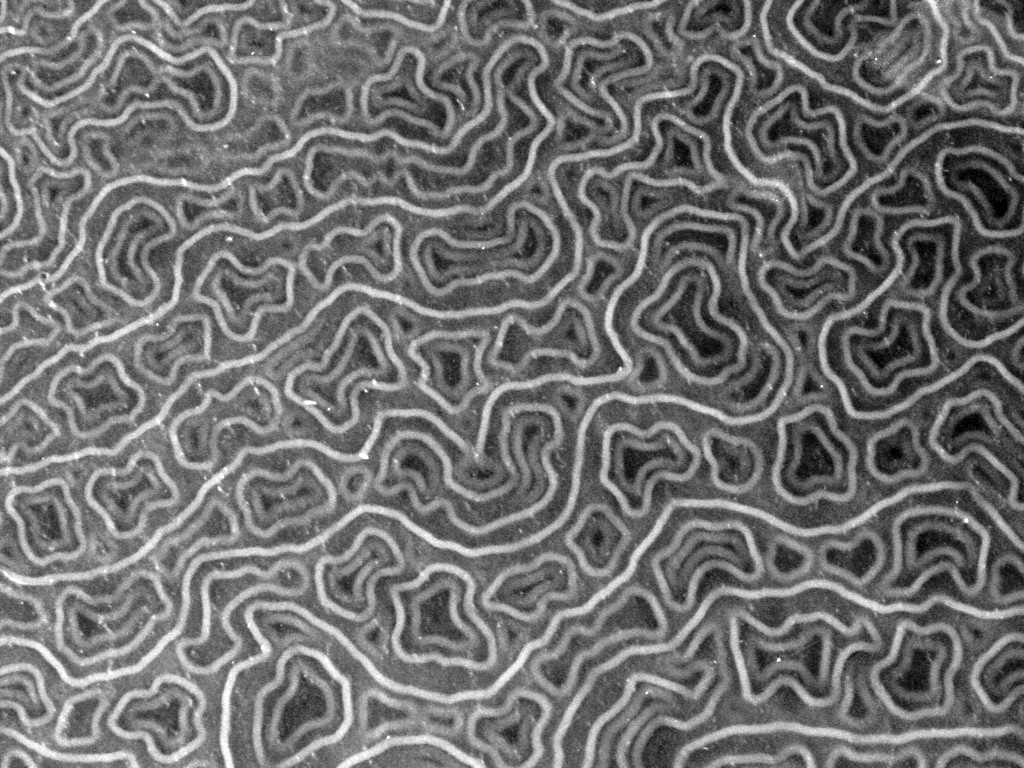
\includegraphics{cas3p2_fluo0p8_GDL4_50um_coating_2_zoom6}};
	\node at (b.north east) (c) {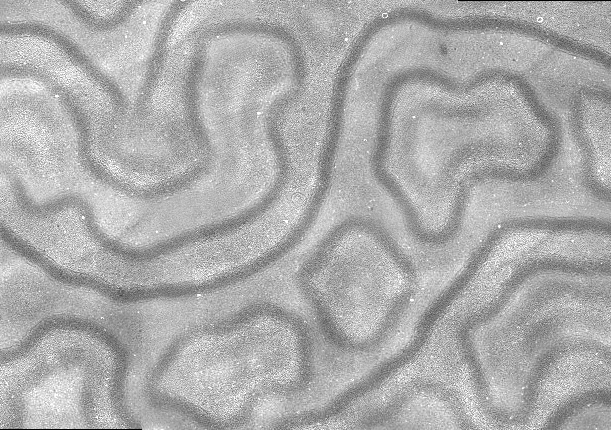
\includegraphics[height=65mm]{cas3p2_fluo0p8_GDL4_50um_coating_2_transmission}};
	\draw[Accent2] (36.4mm, -25mm) rectangle +(28.9mm,-21.7mm);
	\draw[Main] (b.north west) ++(34mm,-34mm) rectangle +(27mm,-19.7mm);
	\draw[Accent1] (c.south west) ++(29mm,29mm) rectangle +(36mm,36mm);
	%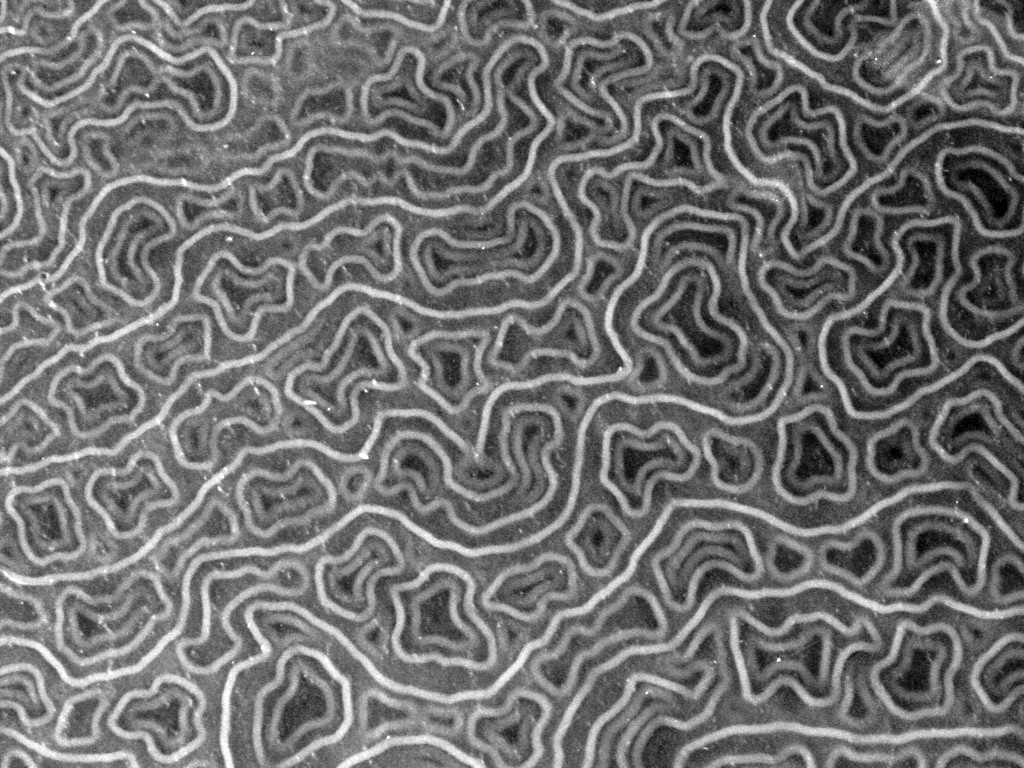
\includegraphics{cas3p2_fluo0p8_GDL4_50um_coating_2_zoom6}
	%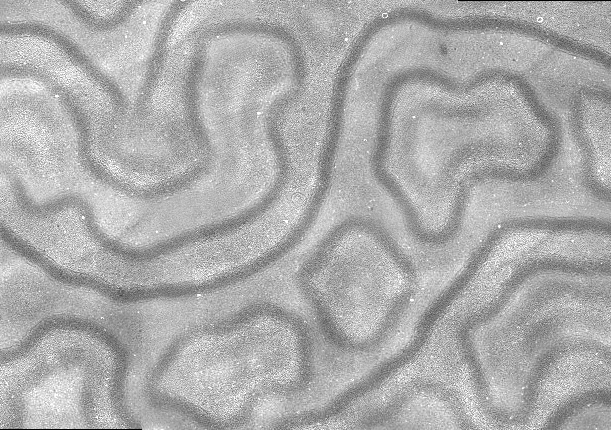
\includegraphics[height=65mm]{cas3p2_fluo0p8_GDL4_50um_coating_2_transmission}
	\end{tikzpicture}

\end{textblock}

\begin{textblock}{3}(8,4.5)
	%\Head{Size distribution}
	
\end{textblock}

\begin{textblock}{7}(0,8)
	\Head{Single-scale tracking\ldots of polydisperse particles}
	
\end{textblock}

\begin{textblock}{3}(8,8)
	\Head{Scale space}
	
\end{textblock}

\begin{textblock}{3}(12,8)
	\Head{Multiscale tracking}
	
\end{textblock}
\begin{textblock}{4}(0,15.85)
\end{textblock}


\begin{textblock}{3.75}(11.25,15.85)
	
\end{textblock}

\begin{textblock}{3}(0,12.1)
	\Head{Buoyancy control}
	\Subhead{by temperature control}
\end{textblock}

\begin{textblock}{7}(4,12.1)
	\Head{Size distributions within local structures}
	
\end{textblock}


\begin{textblock}{15}(0,21.5)
	\Head{Heterogeneous nucleation, Exclusion of small particles \& Formation of grain boundaries}
	
\end{textblock}

\textblockcolour{lightgray!50!white}
\TPMargin*{ 0.125\TPHorizModule }
\begin{textblock}{2.875}(12,2.625)%real width of 3
	\Head{Take away}
	\Subhead{A new kind of wrinkling}
	\begin{itemize}
		\item nested
		\item self generated
	\end{itemize}
	\Subhead{A link with fractures}
\end{textblock}%Conclusion



\end{document}